\section{Presentation Logic Layer}

%What pages will be present in your project? briefly indicate how your website will be organized

\par Wireframing is an essential part of designing a website or application. It refers to the process of creating a visual layout of a webpage or screen, outlining the position and size of each element on the page. By using wireframes, designers can determine the user experience and the complexity of the UI, as well as the content that the user sees. It helps to create a tangible representation of the user interface and provides a clear understanding of how the user interacts with the system.

In our project, we utilized wireframing to design and implement the user interface of our web application. We used wireframes to determine the layout and design of our web pages and to ensure a consistent user experience across the entire application. By using wireframes, we were able to visualize the content and layout of the web pages and make necessary changes before implementing the final design. Our wireframes helped us to create a user-friendly and efficient web application, enhancing the user experience and ensuring the success of our project.

\subsection{Login page}
\begin{figure}[h]
\centering
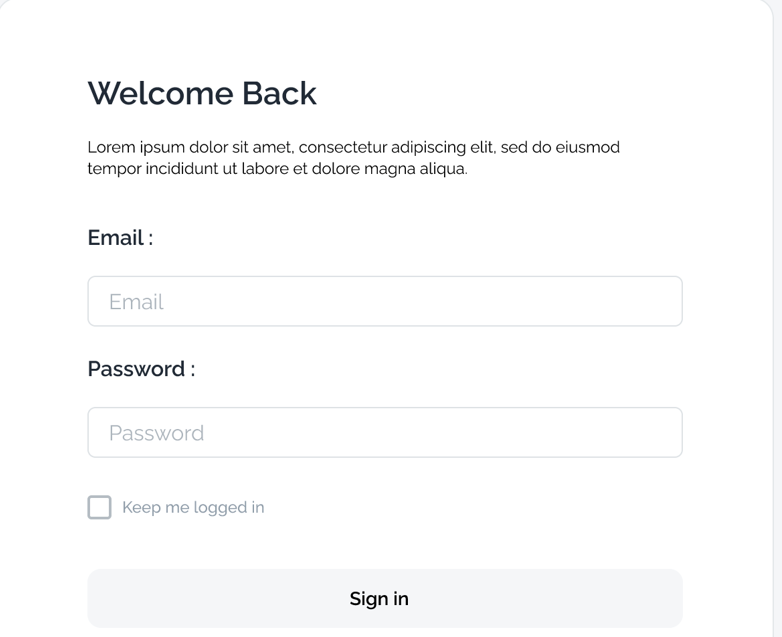
\includegraphics[width=0.5\textwidth]{sections/login_WF.png}
\caption{Login Page}
\label{fig:login}
\end{figure}

The login page of the pharmacy system (Figure~\ref{fig:login}) would likely have two input fields for the user to enter their email address and password. There would also be a "Login" button or similar call-to-action element that the user can click once they have entered their login credentials. This button would submit the form and initiate the authentication process.
\newpage
\subsection{Reciept page}
\begin{figure}[h]
\centering
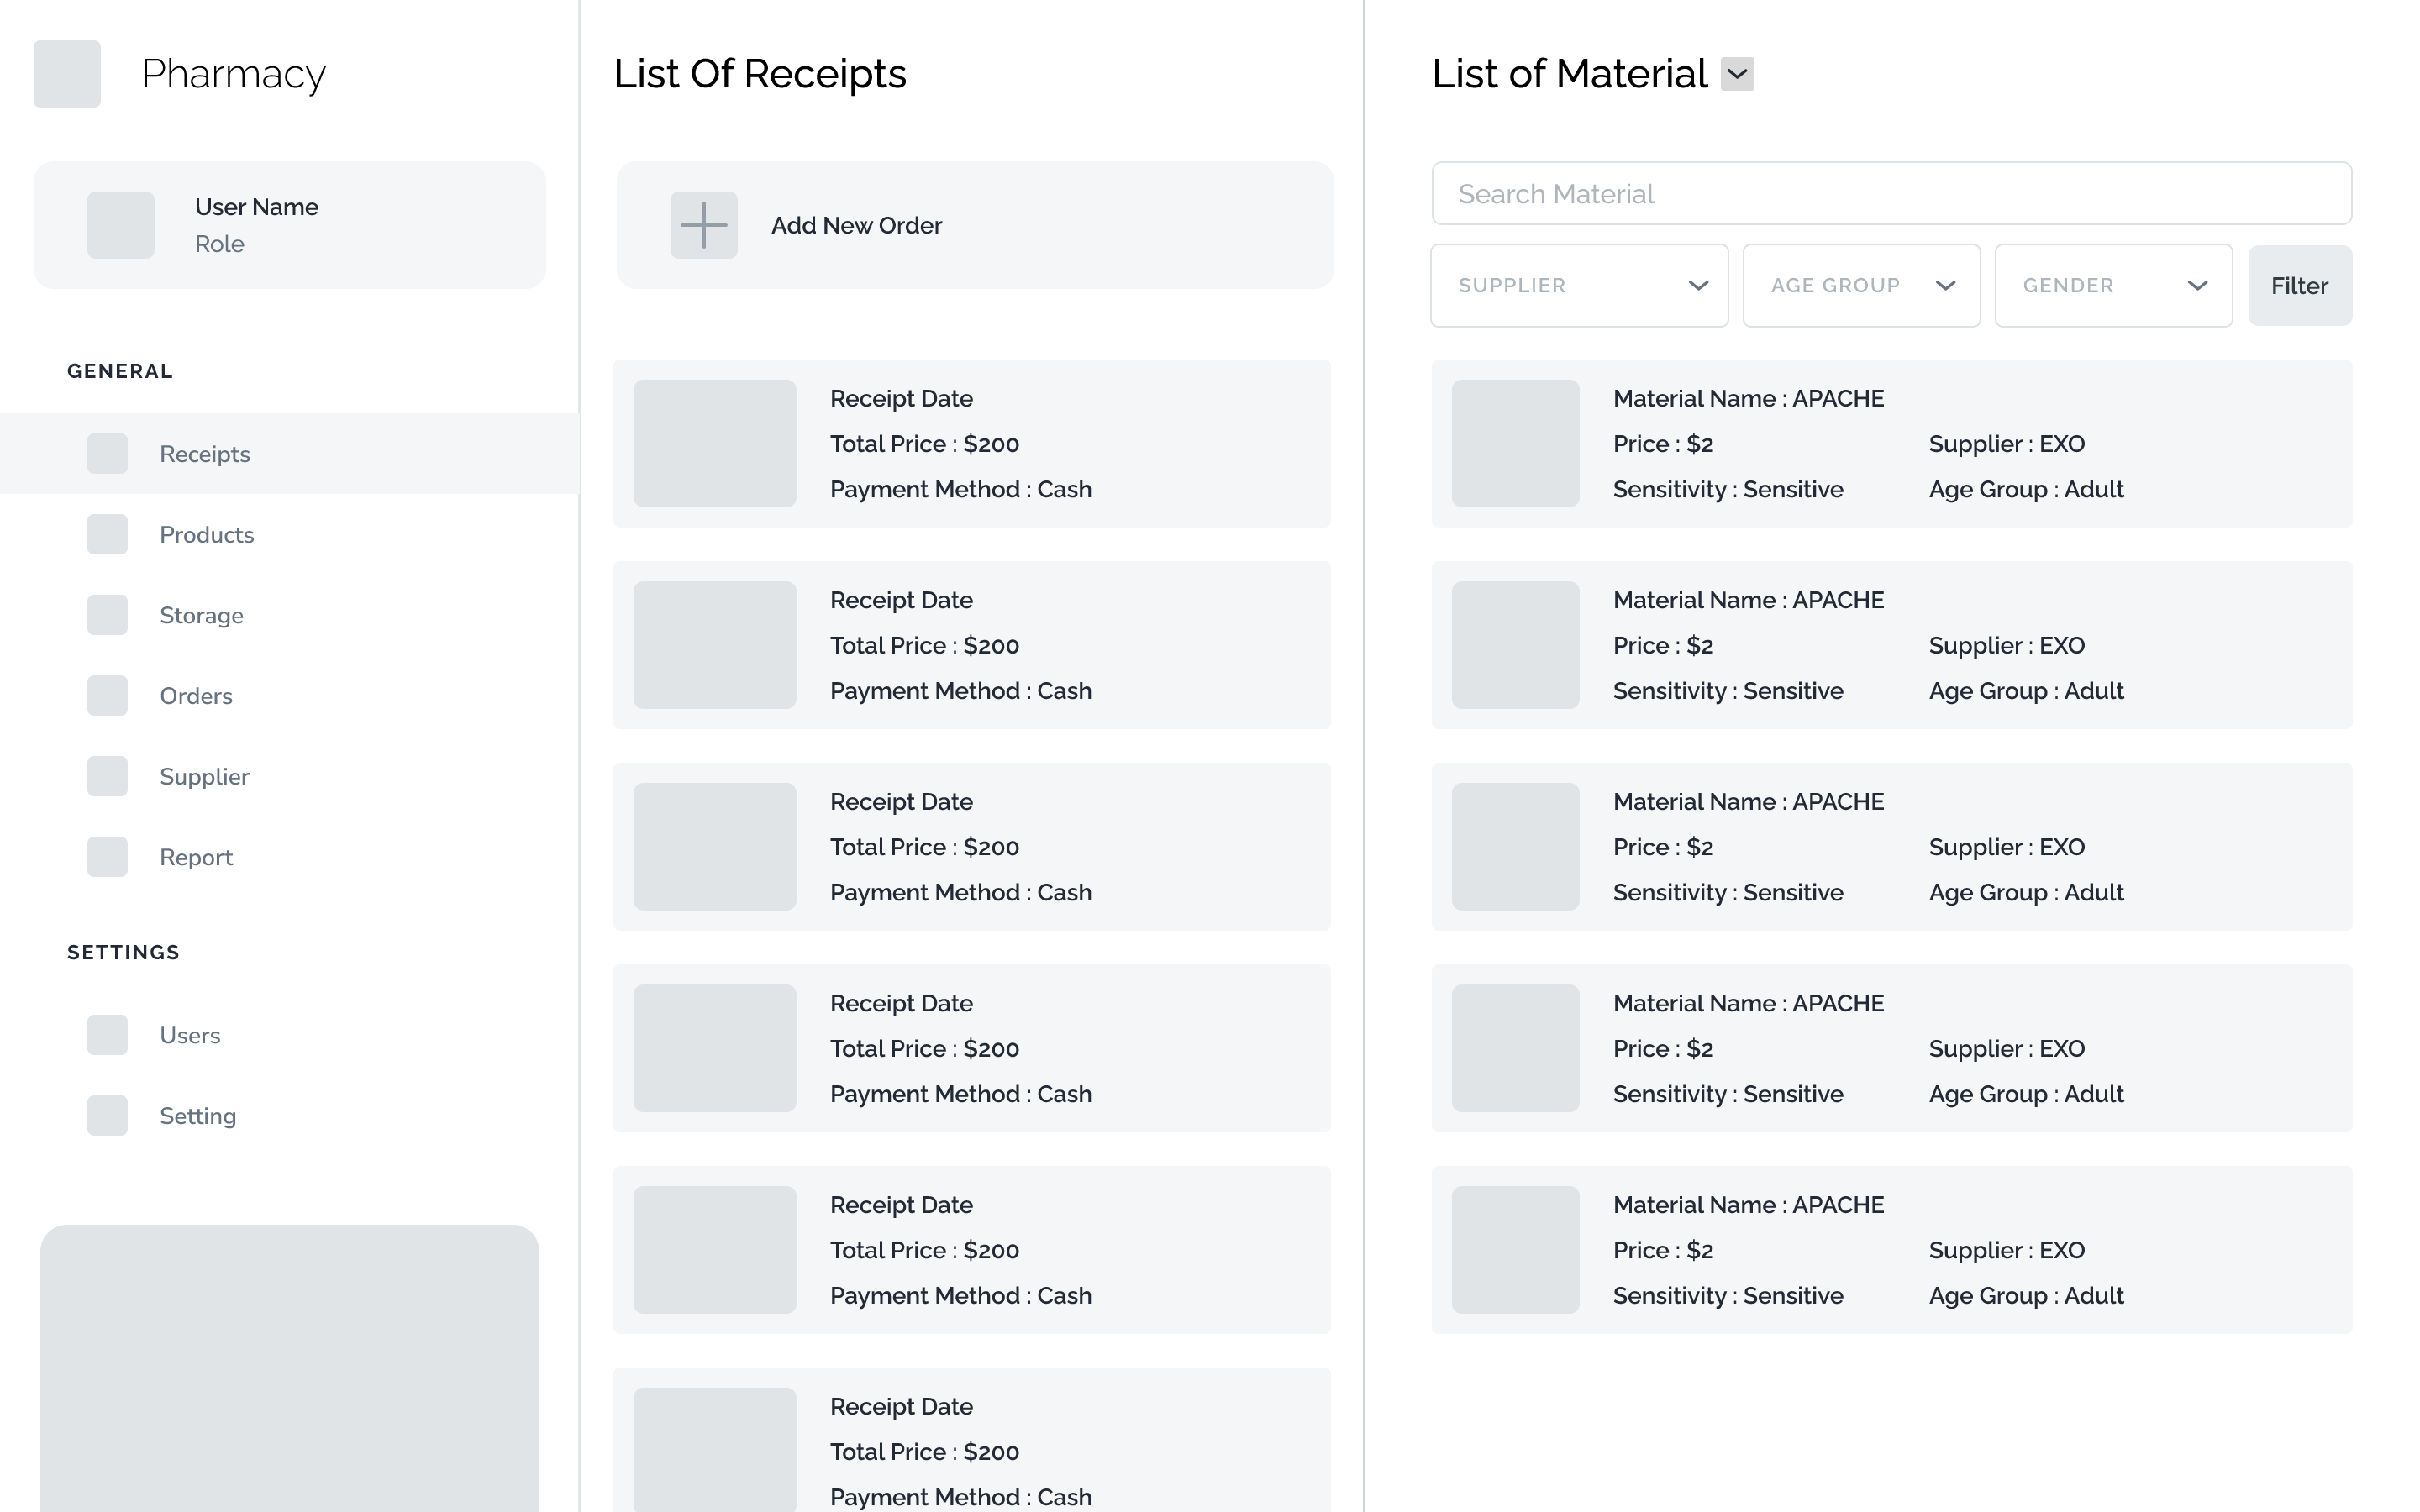
\includegraphics[width=0.8\textwidth]{sections/reciept_WF.png}
\caption{Login Page}
\label{fig:reciept}
\end{figure}
The receipt form (Figure~\ref{fig:reciept}) shows the receipt of a prescription. it may contain drugs or materials or both.